\begin{center}
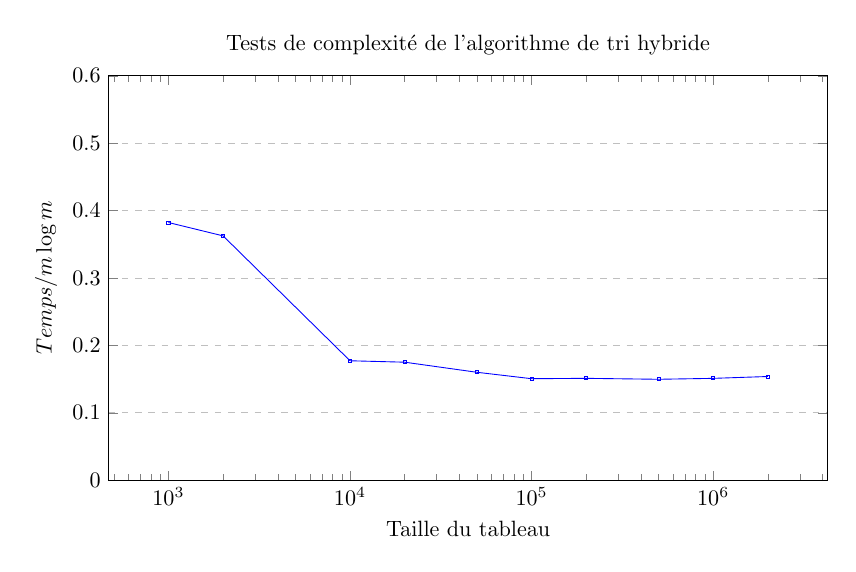
\begin{tikzpicture}[scale=0.8]
\begin{axis}[
    title={Tests de complexité de l'algorithme de tri hybride},
    xlabel={Taille du tableau},
    ylabel={$Temps/m\log m$},
    ymin=0,ymax=0.6,
    legend pos=north west,
    ymajorgrids=true,
    grid style=dashed,
	xmode=log,
	width=13cm,
	height=8cm
]
 
\addplot[
    color=blue,
	mark=square,
	mark size=0.7
    ]
    coordinates {
		(1000,0.382308094493256)(2000,0.362491172251114)(10000,0.177156152448253)(20000,0.175045516984215)(50000,0.1600677813884)(100000,0.150545100831557)(200000,0.151079177559705)(500000,0.149688600266954)(1000000,0.15106237070744)(2000000,0.153803093606565) 
	};
 
\end{axis}
\end{tikzpicture}
\end{center}
